% Created by Ross Barnie
% 
% Please note that I use the Java variable name convention whereby
% each consecutive word in a single variable is capitalised.
%
% This applies to all labels and references

\documentclass[a4paper]{article}

\title{User Guide: Primer Design}

\author{Ross Barnie \\
  Dmitrijs Jonins \\
  Daniel McElroy \\
  Murray Ross \\
  Ross Taylor
}
\date{}

\usepackage{url}
\usepackage{graphicx}
\graphicspath{ {../img/} }

%---------------------------------------------------------------------

\begin{document}
\maketitle
\tableofcontents
\listoffigures
\newpage

%---------------------------------------------------------------------
%---------------------------------------------------------------------

\section{About}
\label{sec:about}

This document will outline how to use the PrimerDesign application
created for use by students of Molecular Methods to learn about
Polymerase Chain Reactions (PCR) and primer design. 

If you encounter any problems while using the application, feel free
to ask your tutor, or email us at \url{TeamProjectQ@gmail.com}.

\section{Getting Started}
\label{sec:gettingstarted}

\subsection{Downloading and Starting the Application}
\label{sec:startingapp}

First, find the \texttt{PrimerDesign.jar} link on the Molecular
Methods moodle site and run it.
You can run it by clicking on the link, however this is dependant on
your browser.
Alternatively, you can save the program to your computer and double
click on it.
If you encounter problems here, ensure that you have Java 6 or newer
installed on your computer.

\subsection{Obtaining a DNA Sequence}
\label{sec:getsequence}

You will need an internet connection to perform these steps.

Now that you have successfully launched the application, you should
prepare a DNA sequence that you wish to manipulate.
As an example, we will show you how to obtain the L1CAM sequence, which
you should already be familiar with, from the NCBI (National Center
for Biotechnology Information) website at
\url{http://www.ncbi.nlm.nih.gov/}.

Use your web browser of choice to go to the NCBI website.
You should see something similar to figure \ref{fig:ncbihome}.

\begin{figure}[h] 
  \begin{center}
    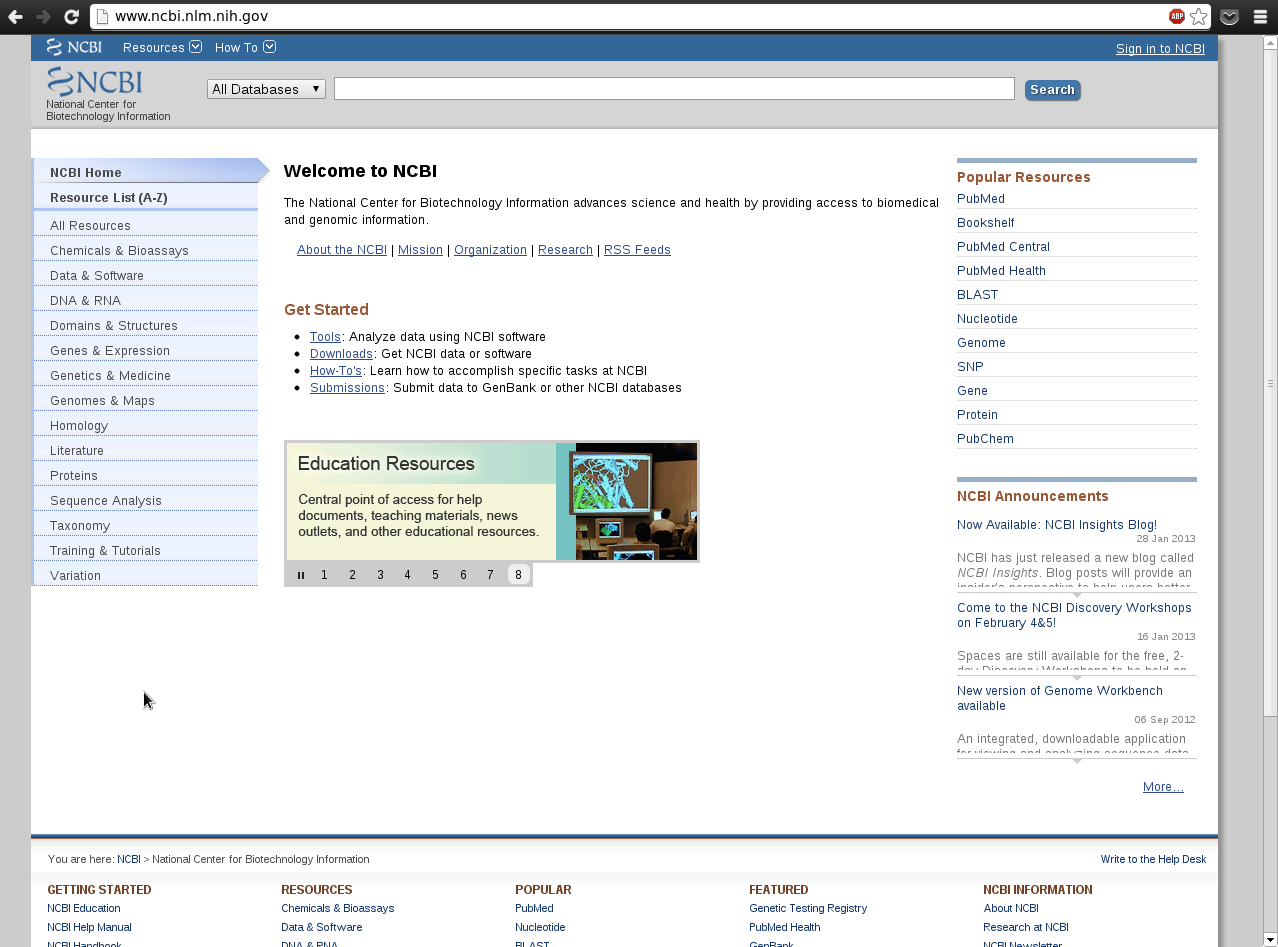
\includegraphics[width=0.8\textwidth]{ncbiHome}
    \caption{\label{fig:ncbihome}NCBI Home Page}
  \end{center}
\end{figure}

In order to search for a compatible sequence, change the search type
to ``Nucleotides'' from the drop-down menu next to the search bar
(highlighted in yellow in figure \ref{fig:ncbihomesearch}) and search
for the sequence you want, for our example this is ``\verb�L1CAM�'',
using the search bar (highlighted in red in figure
\ref{fig:ncbihomesearch}).

\begin{figure}[t]   
  \begin{center}
    
\includegraphics[width=\textwidth]{ncbiHomeSearch}
    \caption{Searching for a sequence\label{fig:ncbihomesearch}}
  \end{center}
\end{figure}

Now you will be presented with your search results, if you are
following our example click on the link highlighted in
yellow on figure \ref{fig:ncbisearchresults}.

\begin{figure}[t]
  \begin{center}
    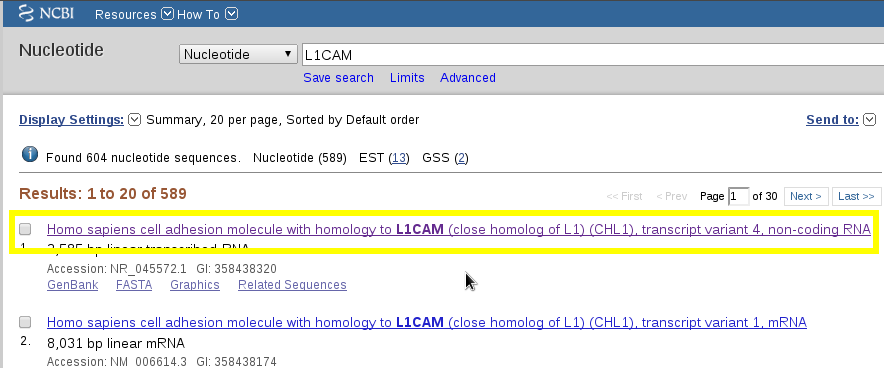
\includegraphics[width=\textwidth]{ncbiSearchResults}
    \caption{\label{fig:ncbisearchresults}Search Results}
  \end{center}
\end{figure}

Once clicked, you should be presented with something similar to figure
\ref{fig:ncbiSequenceSelected}.

\begin{figure}[t]
  \begin{center}
    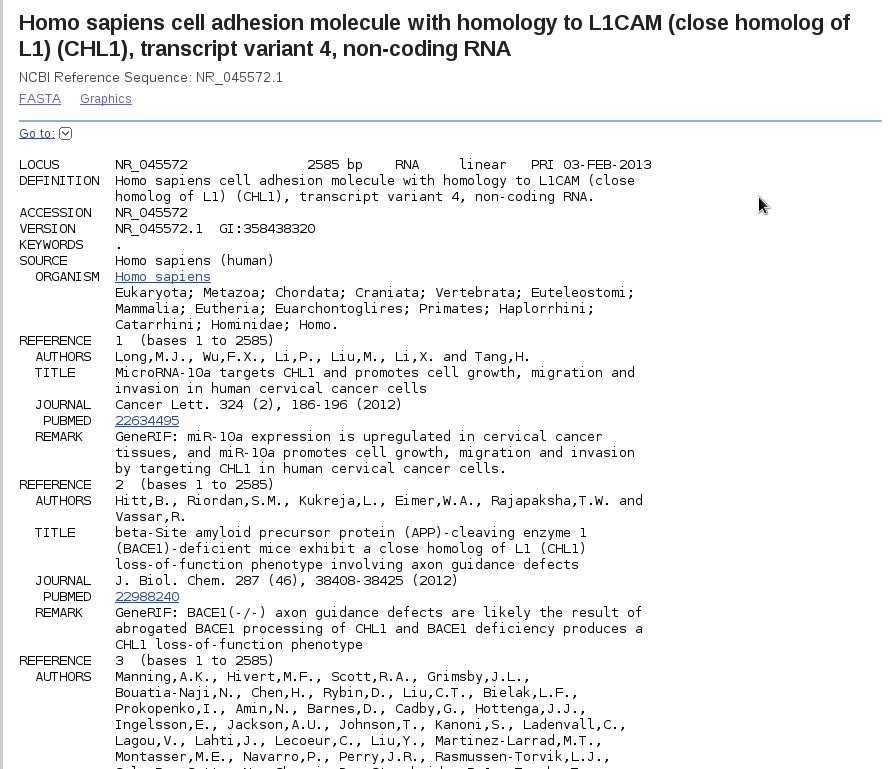
\includegraphics[width=0.8\textwidth]{ncbiSequenceSelected}
    \caption{\label{fig:ncbiSequenceSelected}Sequence Page}
  \end{center}
\end{figure}

Most of this information is irrelevant to this application, so scroll
down until you see the DNA sequence, in our example it should look
like figure \ref{fig:ncbiSequenceFound}.
Now you can simply highlight the sequence (highlighted in yellow in
figure \ref{fig:ncbiSequenceFound}) and press Ctrl-c (or equivalent)
to copy the sequence.

\begin{figure}[t]
  \begin{center}
    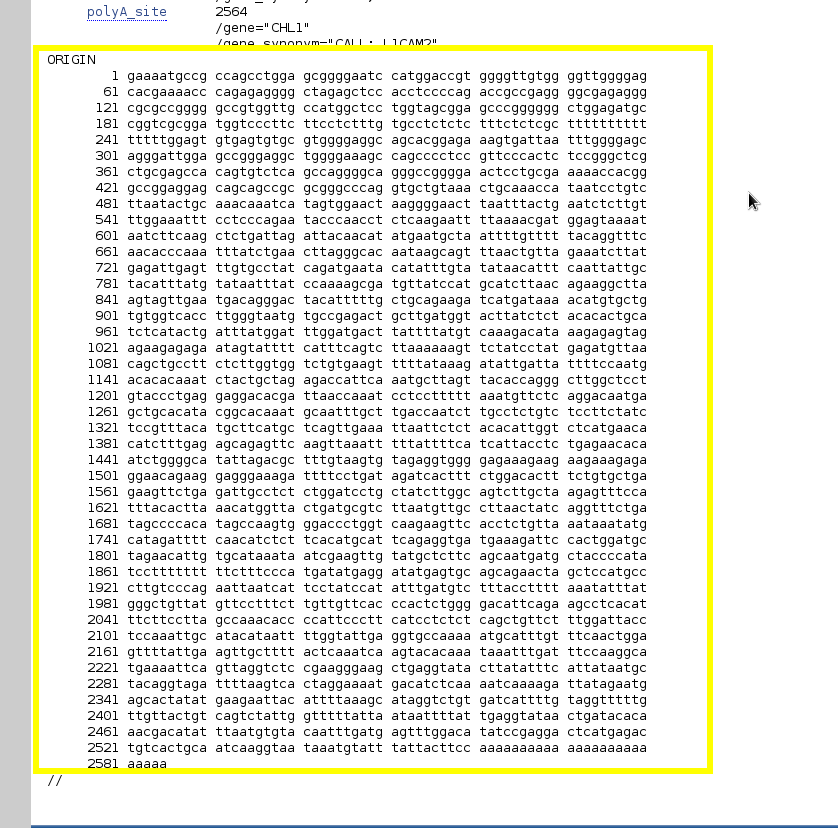
\includegraphics[width=0.8\textwidth]{ncbiSequenceFound}
    \caption{\label{fig:ncbiSequenceFound}The Sequence}
  \end{center}
\end{figure}

%--------------------------------------------------------------------
%--------------------------------------------------------------------

\section{The Application}
\label{sec:theApp}

Please note: the following information and screenshots are subject to
change and may not necessarily reflect the current build of the
system. 
Use your best judgement where differences appear.

%---------------------------------------------------------------------
\subsection{Overview Screen}
\label{sec:overviewScreen}

On starting the application (as described in section
\ref{sec:startingApp}), you should see the overview screen (figure
\ref{fig:PDSplash}) with a button on the bottom right labelled
``Start''. Once you have finished reading the information on this
page, you should press start.

\begin{figure}[t]
  \begin{center}
    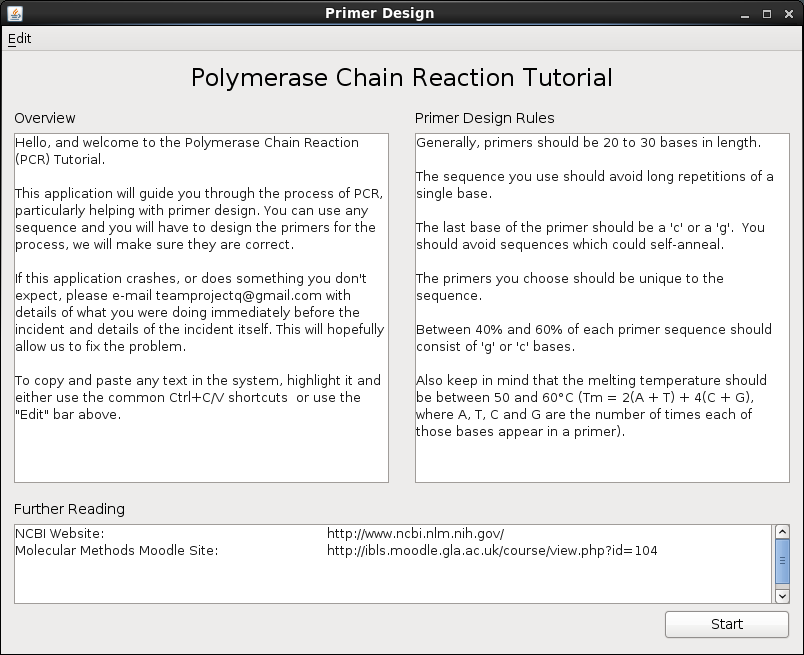
\includegraphics[width=0.8\textwidth]{StartPanel}
    \caption{\label{fig:PDSplash}Overview Screen}
  \end{center}
\end{figure}

%---------------------------------------------------------------------

\subsection{Sequence Entry}
\label{sec:sequenceEntry}

Remember the DNA sequence you copied in section
\ref{sec:gettingSequence}? Well now is the time to paste it!
Simply paste (using Ctrl-V or using the Edit->Paste menu) the sequence
into the large white area and press the next button.
As you can see in figure \ref{fig:PDStartWithSeq}, you do not need to
worry about including the ``ORIGIN'' from the sequence as this will be
removed when you press the `Next' button.

\begin{figure}[t]
  \begin{center}
    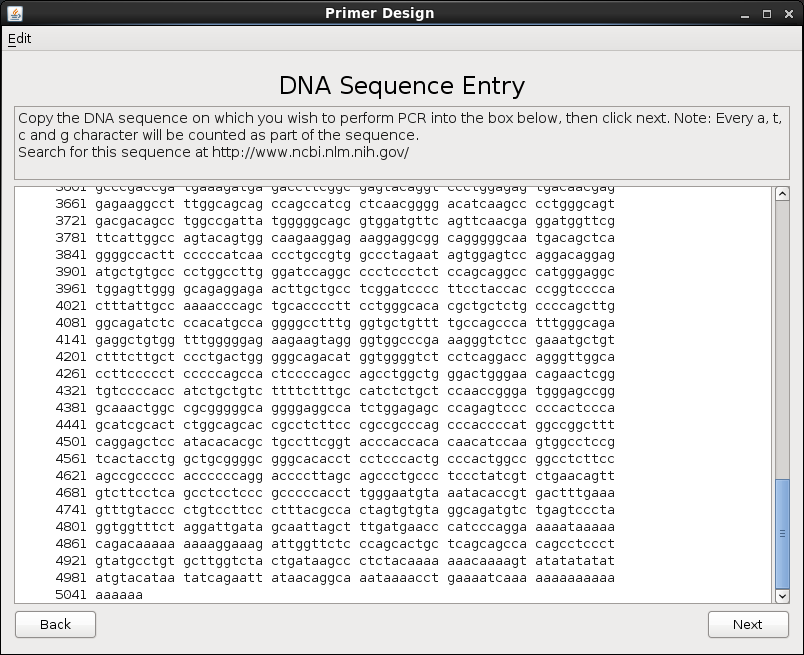
\includegraphics[width=0.8\textwidth]{SequenceEntry}
    \caption{\label{fig:PDStartWithSeq}DNA Sequence Entry Example}
  \end{center}
\end{figure}

%---------------------------------------------------------------------

\subsection{Target Area Selection}
\label{sec:targetAreaSelection}

Now we have to select what it is we want to produce from the reaction.
To do this, you have to specify the first and the last base of the
sequence you wish to copy, using it's position in the sequence.
So if you wish to copy a sequence from position 100 to 500, as in the
example on figure \ref{fig:PDAreaSelection}, you would enter these
into the ``From'' and ``To'' text boxes.
An easier way to do this is to highlight the sequence you wish to use
and the numbers will be filled in for you.

Note that you can also view the complementary strand, by using the
tabs just above where the sequence is.

\begin{figure}[t]
  \begin{center}
    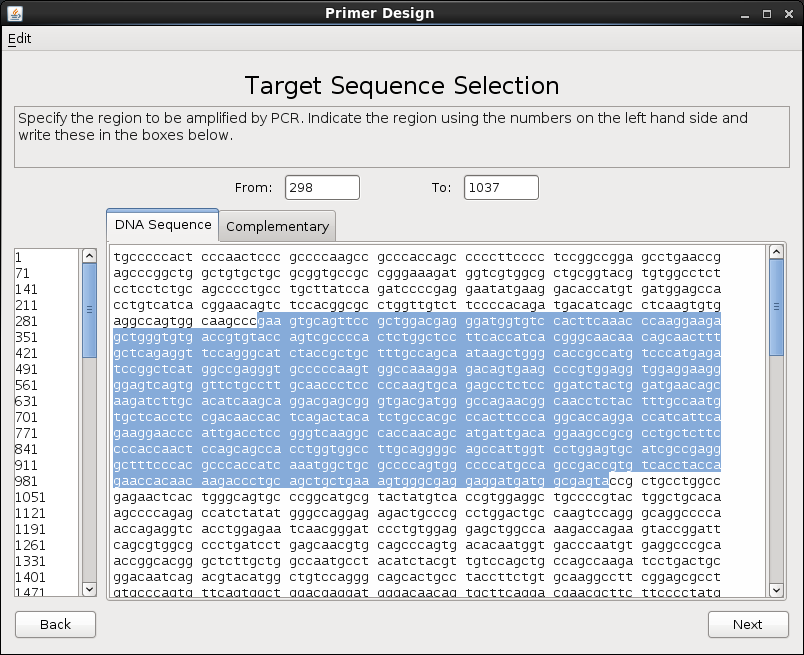
\includegraphics[width=0.8\textwidth]{TargetSelection}
    \caption{\label{fig:PDAreaSelection}Target Area Selection Example}
  \end{center}
\end{figure}

%---------------------------------------------------------------------

\subsection{Primer Design}
\label{sec:primerDesign}

You can now see your selected area more clearly and, since primers can
include bases from before and after the target, the rest of the
sequence is still available to you.

You should design your primers and insert them into the ``Forward Primer''
and ``Reverse Primer'' fields, as shown in figure
\ref{fig:PDPrimerSelection}, note however that the example data is not
designed to be correct.

As you type in a primer, you will notice that what you type is
highlighted in the sequence (as long as you are viewing the correct
strand).
A red highlight corresponds to a primer with at least one rule broken
to an ``unacceptable'' degree, which means that you cannot proceed.

A yellow highlight corresponds to a primer with at least one rule
broken to an ``acceptable'' degree, which will (after 3 attempts)
allow you to proceed if you are absolutely sure you want to continue.

A blue highlight means that you have found a primer which meets all
the requirements and may continue.

For the reverse primer, there is an additional text box which will
reverse the order of the primer you enter, so you should enter the
primer in the 3'---5' direction.
The 5'---3' primer is the one which is checked against the rules.

So if you were to enter \verb�aattccggt�, the additional text box
would show \verb�tggccttaa�.

You can also see the primer design rules again by pressing the ``Show
Primer Design Rules'' button.

You can check your primers individually against the primer design
rules by using the ``Check Primer'' buttons on the bottom of the
window.
These will give you information on where your primers pass and where
they fail.

\begin{figure}[t]
  \begin{center}
    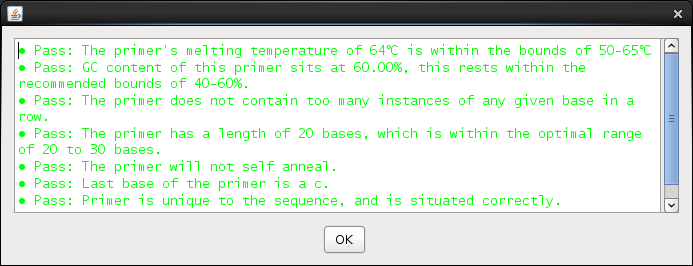
\includegraphics[width=0.8\textwidth]{PrimerAllCorrect}
    \caption{\label{fig:PDPrimerSelection}Primer Selection Example}
  \end{center}
\end{figure}

When you click next, both primers are checked against the rules
described at the start of the application, and you are given a report
of where your primers pass and where they fail, if at all.
This will look something like \ref{fig:PDPrimerFeedback}.

\begin{figure}[t]
  \begin{center}
    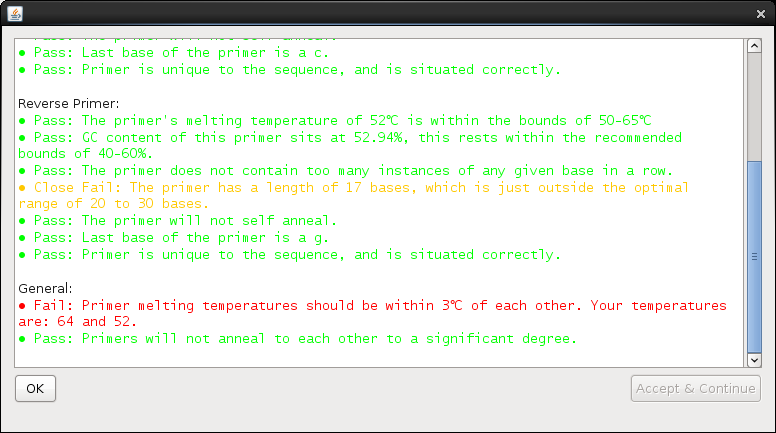
\includegraphics[width=0.8\textwidth]{PrimerFeedback}
    \caption{\label{fig:PDPrimerFeedback}Primer Design Feedback Example}
  \end{center}
\end{figure}

Pressing the ``Ok'' button will close this window and allow you to
continue only if you have passed each rule.
If you have any ``Close Fail'' items in the report, you will only be
allowed to proceed when you have clicked the ``Next'' button another
two times, which will give you the option to ``Accept and Continue''.

%---------------------------------------------------------------------

\subsection{Melting Temperature}
\label{sec:meltingTemp}

This screen, which should be similar to figure
\ref{fig:PDMeltingTemp}, lets you review your design, showing the
melting temperatures of both primers and the primers themselves.

Note that for our example we should not have been allowed to get here
due to the feedback we received in figure \ref{fig:PDPrimerFeedback}.

\begin{figure}[t]
  \begin{center}
    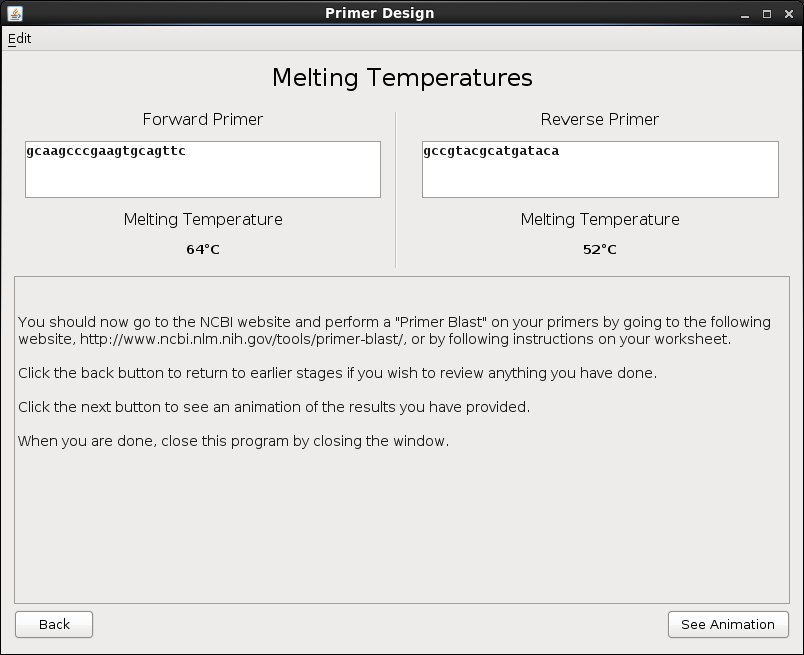
\includegraphics[width=0.8\textwidth]{Temperature}
    \caption{\label{fig:PDMeltingTemp}Melting Temperature Screen Example}
  \end{center}
\end{figure}


%---------------------------------------------------------------------
%---------------------------------------------------------------------

\section{Known Bugs}

There are a few known issues with the current build of the
system.
These are constantly changing with the development of the application
so are not listed here.
If you suspect you have found something which should not have, please
feel free to e-mail us at \texttt{TeamProjectQ@gmail.com}.
